\section{Velvet NIPoPoWs}\label{sec:construction}
In order to eliminate the Chainsewing Attack we propose an update to the velvet NIPoPoW protocol. The core problem is that, in her suffix proof, the adversary was able to claim not only blocks of shorter forked chains, but also arbitrarily long parts of the chain adopted by an honest party. Since thorny blocks are accepted as valid, the verifier cannot distinguish blocks that actually belong in a chain from blocks that only seem to belong in the same chain because they are pointed to from a thorny block.

The idea for a secure protocol is to distinguish the smooth from the thorny blocks, so that smooth blocks can never point to thorny blocks. In this way we can make sure that thorny blocks acting as passing points to fork chains, as block $a'$ does in Figure \ref{fig:attack}, cannot be pointed to by honestly generated blocks. Therefore, the adversary cannot utilize honest mining power to construct a stronger suffix proof for her fork chain. In order to formally describe the suggested protocol patch, we first define the notion of a smooth interlink pointer.

\begin{definition}[Smooth Pointer]
  A \emph{smooth pointer} of a block $b$ for a specific level $\mu$ is the interlink pointer to the most recent $\mu$-level smooth ancestor of $b$.
	\label{defn:smooth_pointer}
\end{definition}

We describe a protocol patch that operates as follows. The superblock NIPoPoW protocol works as usual but each miner constructs smooth blocks. This means that  a block's interlink is constructed excluding thorny blocks. In this way, although thorny blocks are accepted in the chain, they are not taken into consideration when updating the interlink structure for the next block to be mined. No honest block could now point to a thorny superblock that may act as the passing point to the fork chain in an adversarial suffix proof. Thus, after this protocol update the adversary is only able to inject adversarially generated blocks from an honestly adopted chain to her own fork.
At the same time, thorny blocks cannot participate in an honestly generated suffix proof except for some blocks in the proof's suffix $(\chi)$. This argument holds because thorny blocks do not form a valid chain along with honestly mined blocks anymore. Consequently, as far as the blocks included in a suffix proof is concerned, we can think of thorny blocks as belonging in the adversary's fork chain for the $\pi$ part of the proof,  which is the comparing part between proofs. Figure~
\ref{fig:injection} illustrates this remark.

\begin{figure}[h!]
	\begin{center}
		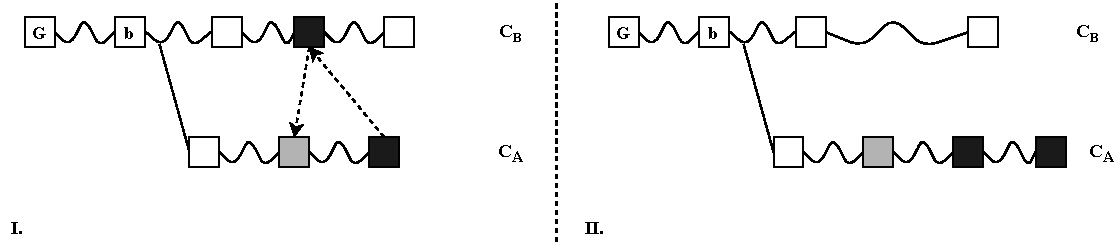
\includegraphics[width=0.9\columnwidth]{figures/injection.pdf}
	\end{center}
	\caption{The adversarial fork chain $\chain_A$ and chain $\chain_B$ of an honest party. Thorny blocks are colored black. Dashed arrows represent interlink pointers. Wavy lines imply one or more blocks. After the protocol update, when an adversarially generated block is sewed from $\chain_B$ into the adversary's suffix proof the verifier conceives $\chain_A$ as longer and $\chain_B$ as shorter. \textbf{I:} The real picture of the chains. \textbf{II:} Equivalent picture from the verifier's perspective considering the blocks included in the corresponding suffix proof for each chain.}
	\label{fig:injection}
\end{figure}

In order to make NIPoPoWs a secure protocol under velvet fork conditions we suggest that the NIPoPoW protocol under velvet fork works as usual but a miner constructs a block's interlink without pointers to thorny blocks.

In order to prove the security of the updated protocol we need to strengthen the Honest Majority Assumption to 1/4 adversary with respect to upgraded honest miners.

\begin{definition}[Velvet Honest Majority]
	Let $n_h$ be the number of upgraded honest miners. Then $t$ out of total $n$ parties are corrupted such that $\dfrac{t}{n_h} < \dfrac{1 - \delta_v}{3} $.
	\label{defn:velvet_honest_majority}
\end{definition}

The following Lemmas come as immediate results from the suggested protocol
update.

\begin{lemma}
	A velvet suffix proof constructed by an honest party cannot contain any thorny block.
	\label{lemm:smooth_honest_suffix}
\end{lemma}

\begin{lemma}
	Let $\mathcal{P_A} = (\pi_\mathcal{A}, \chi_\mathcal{A})$ be a velvet suffix proof constructed by the adversary and block $b_s$, generated at round $r_s$, be the most recent smooth block in the proof. Then $\forall r:r < r_s$ no thorny blocks generated at round $r$ can be included in $\mathcal{P_A}$.
	\label{lemm:smooths_before_smooth}
\end{lemma}
\begin{proof}
By contradiction. Let $b_t$ be a thorny block generated at some round $r_t < r_s$. Suppose for contradiction that $b_t$ is included in the proof. Then, because $\mathcal{P_A}$ is a valid chain as for interlink pointers, there exist a block path made by interlink pointers starting from $b_s$ and resulting to $b_t$. Let $b'$ be the most recently generated thorny block after $b_t$ and before $b_s$ included in $\mathcal{P_A}$. Then $b'$ has been generated at a round $r'$ such that $r_t \leq r' < r_s$. Then the block right after block $b'$ in $\mathcal{P_A}$ must be a thorny block since it points to $b'$ which is thorny. But $b'$ is the most recent thorny block after $b_t$, thus we have reached a contradiction.
\end{proof}

\begin{lemma}
	Let $\mathcal{P_A} = (\pi_\mathcal{A}, \chi_\mathcal{A})$ be a velvet suffix proof constructed by the adversary. Let $b_t$ be the oldest thorny bock included in $\mathcal{P_A}$ which is generated at round $r_t$. Then any block $b = \{b: b \in \mathcal{P_A} \wedge \text{b generated at }r \geq r_t \}$ is thorny.
	\label{lemm:thorny_after_thorny}
\end{lemma}
\begin{proof}
By contradiction. Suppose for contradiciton that $b_s$ is a smooth block generated at round $r_s > r_t$. Then from Lemma \ref{lemm:smooths_before_smooth} any block generated at round $r < r_s$ is smooth. But $b_t$ is generated at round $r_t < r_s$ and is thorny, thus we have reached a contradiction.
\end{proof}

The following corollary emerges immediately from Lemmas \ref{lemm:smooths_before_smooth}, \ref{lemm:thorny_after_thorny}. This result is illustrated in Figure \ref{fig:adversarial_velvet_proof}.

\begin{corollary}
	Any adversarial proof $\mathcal{P_A} = (\pi_\mathcal{A}, \chi_\mathcal{A})$ containing both smooth and thorny blocks consists of a prefix smooth subchain followed by a suffix thorny subchain.
	\label{cor:adversarial_proof_scheme}
\end{corollary}

\begin{figure}[h!]
	\begin{center}
		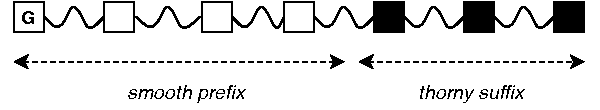
\includegraphics[width=0.9\columnwidth]{figures/adversarial_velvet_proof.pdf}
	\end{center}
	\caption{In the general case the adversarial velvet suffix proof $\mathcal{P_A} = (\pi_\mathcal{A}, \chi_\mathcal{A})$ consists of an initial part of smooth blocks followed by thorny blocks.}
	\label{fig:adversarial_velvet_proof}
\end{figure}
We now describe the algorithms needed by the upgraded miner, prover and verifier. The upgraded miner acts as usual except for including the interlink of the newborn block in the coinbase transaction. In order to construct an interlink containing only the smooth blocks, the miner keeps a copy of the ``smooth chain'' ($\chain_S$) which consists of the smooth blocks existing in the original chain $\chain$. The algorithm for extracting the smooth chain out of $\chain$ is given in Algorithm \ref{alg:smooth_chain_suffix}. Function \textit{isSmoothBlock(B)} checks whether a block \textit{B} is a smooth velvet by calling \textit{isSmoothPointer(B,p)} for every pointer \textit{p} in \textit{B}'s interlink. Function \textit{isSmoothPointer(B,p)} returns \emph{true} if $p$ is a valid pointer, in essence a pointer to the most recent \emph{smooth velvet} for the level denoted by the pointer itself. The \textit{updateInterlink} algorithm is given in Algorithm \ref{alg:updateInterlink}, which is essentially the same as in the case of a hard/soft fork, except for working on the smooth chain $\chain_S$ instead of $\chain$.

The construction of the velvet suffix prover is given in Algorithm \ref{alg:velvet_suffix_prover}, which is essentially the same to that of a hard/soft fork except for working on smooth chain $\chain_S$ instead of $\chain$.

In conclusion the Verify algorithm for the NIPoPoW suffix protocol remains the same as in the case of hard or soft fork.

\begin{algorithm}[H]
	\caption{\label{alg:smooth_chain_suffix}Smooth chain for suffix proofs}
	\begin{algorithmic}[1]
			\Function{\sf smoothChain}{$\chain$}
				\Let{\chain_S}{\{\mathcal{G}\}}
				\Let{k}{1}
				\While{$\chain[-k] \neq \mathcal{G}$}
						\If{$\textsf{isSmoothBlock}(\chain[-k])$}
							\Let{\chain_S}{\chain_S \cup \chain[-k]}
						\EndIf
						\Let{k}{k + 1}
				\EndWhile
				\State\Return{$\chain_S$}
			\EndFunction
	\end{algorithmic}
	\vspace{4mm}
	\begin{algorithmic}[1]
			\Function{\sf isSmoothBlock}{$B$}
				\If{$B = \mathcal{G}$}
					\State\Return{$\true$}
				\EndIf
				\For{$p \in B.\textsf{interlink}$}
						\If{$\lnot \textsf{isSmoothPointer}(B, p)$}
							\State\Return{$\false$}
						\EndIf
				\EndFor
				\State\Return{$\true$}
			\EndFunction
	\end{algorithmic}
	\vspace{4mm}
	\begin{algorithmic}[1]
			\Function{\sf isSmoothPointer}{$B, p$}
				\Let{b}{\textsf{Block}(B.\textsf{prevId})}
				\While{$b \neq p$}
						\If{$\textsf{level}(b) \geq \textsf{level}(p) \land \textsf{isSmoothBlock}(b)$}
							\State\Return{$\false$}
						\EndIf
						\If{$b = \mathcal{G}$}
							\State\Return{$\false$}
						\EndIf
						\Let{b}{\textsf{Block}(b.\textsf{prevId})}
				\EndWhile
				\State\Return{$\textsf{isSmoothBlock}(b)$}
			\EndFunction
	\end{algorithmic}
\end{algorithm}

\begin{algorithm}[h!]
		\caption{\label{alg:updateInterlink}Velvet updateInterlink}
		\begin{algorithmic}[1]
				\Function{\sf updateInterlinkVelvet}{$\chain_S$}
						\Let{B'}{\chain_S[-1]}
						\Let{\textsf{interlink}}{B'.\textsf{interlink}}
						\For{$\mu = 0$ to $\textsf{level}(B')$}
								\Let{\textsf{interlink}[\mu]}{\textsf{id}(B')}
						\EndFor
						\State\Return$\textsf{interlink}$
				\EndFunction
		\end{algorithmic}
\end{algorithm}

\begin{algorithm}[h!]
		\caption{\label{alg:velvet_suffix_prover}Velvet Suffix Prover}
		\begin{algorithmic}
				\Function{\sf ProveVelvet$_{m,k}$}{$\chain_S$}
					\Let{B}{\chain_S[0]}
					\For{$\mu = \lvert \chain_S[-k].\textsf{interlink} \rvert$ down to $0$}
						\Let{\alpha}{\chain_S[{:}-k]\{B{:}\}\upchain^\mu}
						\Let{\pi}{\pi \cup \alpha}
						\Let{B}{\alpha[-m]}
					\EndFor
					\Let{\chi}{\chain_S[-k{:}]}
					\State\Return$\pi\chi$
				\EndFunction
		\end{algorithmic}
\end{algorithm}
